% !TEX encoding = UTF-8 Unicode
\documentclass[handout]{beamer}
\usepackage[frenchb]{babel}
\usepackage[T1]{fontenc}
\usepackage[utf8]{inputenc}

% functions to plot
\def\func(#1){(#1)*(1-(#1))}
\hypersetup{colorlinks = true,linkcolor = blue,urlcolor  = blue}

\newenvironment{iPar}[1]{\textbf{#1} \begin{itemize}}{\end{itemize}}

\title{Math Boot Camp}
\author{Microeconomics \\ 20851}
\date{}

\begin{document}

\frame{\titlepage}

\section[Outline]{}
\frame{\tableofcontents}

\section{Introduction}
\frame
{
  \frametitle{Microeconomics}
Your micro courses to date
  \begin{itemize}
  \item<1-> Microeconomics 1-851-07
  \item<2-> Econ. Problems and Policy Analysis, 2-851-07
  \end{itemize}
  \vspace{0.2in}
  Micro is central to Economics: 
  \begin{itemize}
    \item<3-> Macro leans heavily on micro (more and more)...
    \item<4-> Micro integrates concepts from psychology and sociology
    \item<5-> Artificial intelligence can use micro
  \end{itemize}
}

\begin{frame}{Microeconomists and inequality}

\begin{figure}
	
\includegraphics[scale=0.35]{justice.png}
	\caption{Take a look at \href{https://missingprofits.world/}{missingprofits.world} to see an estimation of what each country loses to tax heavens}
\end{figure}

\end{frame}


\begin{frame}{Microeconomists and the climate}

\begin{figure}
	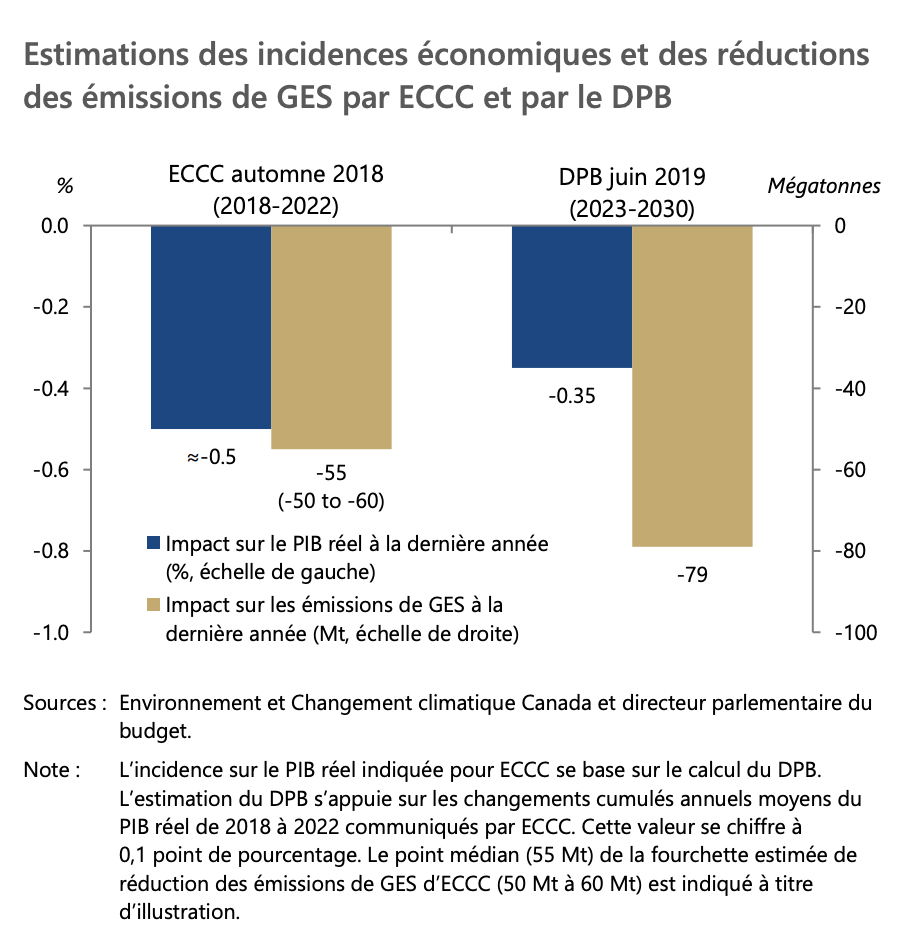
\includegraphics[scale=0.35]{climat.png}
	\caption{The Parlamentary Budget Officer - 2019}
\end{figure}

\end{frame}


\begin{frame}{The new economy}

\begin{figure}
	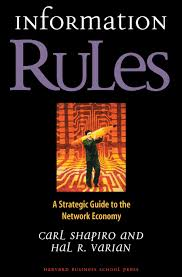
\includegraphics[scale=0.5]{rules.jpeg}
	\caption{Hal Varian is the chief economist at Google}
\end{figure}

\end{frame}

\begin{frame}{Microéconomists at AirBnB}

\begin{figure}
	
\includegraphics[scale=0.25]{AI.png}
	\caption{The Economist, 2015}
\end{figure}

\end{frame}




\begin{frame}{Data: The crux of the matter}

Data is everywhere. Theory helps out make sense out of it:

  \begin{itemize}
  \item<1-> Understanding behaviours (e.g. testing theories)
  \item<2-> Quantifying effects to form normative and positive judgements about policies
  \item<3-> Tarification and optimization within a firm
  \item<4-> It's dangerous to use data without a theoretical frame (see this \href{https://www.quantamagazine.org/to-build-truly-intelligent-machines-teach-them-cause-and-effect-20180515/}{article} on artificial intelligence)
  \end{itemize}

\end{frame}

\section{Course structure}

\begin{frame}{The themes we will cover}
  \begin{itemize}
  \item<1-> Consumption
  \item<2-> Markets and welfare
  \item<3-> Production decisions
  \item<4-> Strategic behaviour
  \item<5-> Auctions
  \end{itemize}
  
\end{frame}

\begin{frame}{Evaluation}

\begin{itemize}
\item 1 Individual assignment (5\%)
\item 3 Group assignments (30\%)
\item Midterm (25\%) and Final (40\%)
\end{itemize}

\end{frame}

\begin{frame}{Other points}

\begin{itemize}
\item Teacher assistant: Nicholas Trottier-Lacourse
\item Reference (non-mandatory) for this course:
\begin{itemize}
    \item Hal Varian (2009). \textit{Intermediate Microeconomics}
\end{itemize}
\item Theory and practice (programming on Google Collab)
\end{itemize}

\end{frame}

\section{Math boot camp}

\begin{frame}{Marginal analysis and approximations}

Linear approximation:

\begin{itemize}\item Functions are generally complicated, but linear functions are simple...
\item Locally, we can approximate any "smooth" function at $x_0$, for  a given $x$ near $x_0$: 
\begin{eqnarray*} 
	f(x) \simeq f(x_0) + \alpha (x-x_0) + ...  
\end{eqnarray*}
\end{itemize}
\textbf{Exercise A}: Graphically illustrate a first-order approximation.
\end{frame}

\begin{frame}{Link with derivatives}
Given $x$ near $x_0$
\begin{align*}
&f(x) \simeq f(x_0) + \alpha (x-x_0) \\ \\ \iff & f(x) -f(x_0) \simeq \alpha (x-x_0)\\\\
 \iff & \alpha \simeq \frac{f(x) -f(x_0)}{x-x_0}  \simeq\; f'(x_0) \quad \text{by definition}
\end{align*}
\pause
Thus  \begin{align*}&f(x) \simeq f(x_0) + f'(x_0) (x-x_0) \quad \text{ or }\\ \\ &f(x) - f(x_0) \simeq f'(x_0) (x-x_0) \quad \text{ or } \\ \\
&\Delta f \simeq f'(x_0) \Delta x
\end{align*}

\end{frame}

\begin{frame}{General derivatives}

\begin{columns}
\footnotesize
\begin{column}{0.5\textwidth}
   With constants
   \begin{itemize}
   		\item $f(x) = b + ax$: $f'(x) = a$
		\item $f(x) = \log x$: $f'(x) = \frac{1}{x}$
		\item $f(x) = e^{ax}$: $f'(x) = ae^{ax}$ 
		\item $f(x) = x^a$: $f'(x) = a x^{a-1}$
   \end{itemize}
\end{column}
\begin{column}{0.5\textwidth}  %%<--- here
	With functions
	\begin{itemize}
		\item $f(x) = a(x)b(x)$, $f'(x) = a'(x)b(x) + a(x)b'(x)$
		\item $f(x) = \frac{a(x)}{b(x)}$, $f'(x) = \frac{a'(x)b(x) - a(x)b'(x)}{b(x)^2}$
		\item $f(x) = a(b(x))$, $f'(x) = a'(b(x))b'(x)$
		\item $f(x) = a(x) + b(x)$, $f'(x) = a'(x) + b'(x)$. 
	\end{itemize}
\end{column}
\end{columns}
\vspace{0.5in}
\textbf{Exercise B}: Find the derivatives of : $f(x)=\sqrt{x},\frac{x}{1+x},\frac{1}{2}x^2 + 2x-10,(1+\frac{x}{2})^2$.
\end{frame}


\begin{frame}{Higher order approximations}

We can take this method further
\begin{itemize}
\item A simple second-order polynomial...
\item Therefore, we use a second-order approximation
\item $k$-order polynomial \ldots
\end{itemize}\
\pause
This is called a Taylor approximation. This has to do with higher-order derivatives of a function:
\begin{eqnarray*}
	f(x) = f(x_0) + f'(x_0)(x-x_0) +\frac{1}{2}f''(x_0)(x-x_0)^2 + \ldots 
\end{eqnarray*}
Written $f'(x), f''(x)$ or $\frac{d f}{d x},\frac{d}{d x}(\frac{d f}{d x}) = \frac{d^2 f}{d x^2} $.
\end{frame}

\begin{frame}{Concavity and Convexity of functions}

A function is convex if for every point $(x_1,x_2)$ and every $0<\lambda<1$: 
\begin{align*}
f(\lambda x_1 + (1-\lambda) x_2) \leq \lambda f(x_1) + (1-\lambda)f(x_2)
\end{align*}

and concave if the opposite is true. We say "strictly" if the inequalities are strict. 

\end{frame}



\begin{frame}{Approximation and maximization (without constraints)}

Consider a first order approximation:
\begin{eqnarray}
 f(x_0+\Delta x) \simeq f(x_0)+ f'(x_0)\Delta x 
\end{eqnarray}

Notice:
\begin{itemize}
\item If $f'(x_0)>0$  a small change $\Delta x>0$ increases $f$
\item If $f'(x_0) <0$ a small change $\Delta x <0$ increases $f$
\item If $x_0$  is the solution to  $\max_x f(x)$, therefore $f'(x_0) =0$
\end{itemize} 
\end{frame}

\begin{frame}{Maximizing without constraints}

Consider a second order approximation:
\begin{eqnarray}
 f(x_0+\Delta x) \simeq f(x_0) + f'(x_0)\Delta x +\frac{1}{2}f''(x_0)\Delta x ^2  
\end{eqnarray}

For a local maximum, we need $f'(x_0)=0$ (FOC) and $f''(x_0)<0$ (SOC). 
Notice that:
\begin{itemize}
\item If $f'(x_0) = 0$ but $f''(x_0)>0$, then $f(x_0+\Delta x) > f(x_0)$. 
\item f'(x) must be positive when $\Delta x <0$ and negative when $\Delta x>0$. 
\end{itemize}

\textbf{Exercise C}: Graphically show the optimum of a concave function.
\end{frame}


\begin{frame}{The envelope theorem}

Take the function $f(x,p)$ in which $p$ is out of our control (exogenous). We denote:

\begin{eqnarray*}
 V(p) = \max_x f(x,p) , \quad x^*(p) = \arg \max_x f(x,p)
\end{eqnarray*}

We then have $V(p) = f(x^*(p),p)$. Thus, 

\begin{eqnarray}
V'(p) = f'_x(x^*(p),p)x^{*'}(p) + f'_p(x^*(p),p)
\end{eqnarray}
However, because $x^*(p)$ maximizes $f(x,p)$, $f'_x(x^*(p),p) = 0$ by definition. This means, $V'(p) = f'_p(x^*(p),p)$.  

\textbf{Exercise D}: Show the value of this approximation for $V(p) = (10 - p\frac{x}{2})x$. 
\end{frame}

\begin{frame}{Constrained maximization}

Consider this problem: 
\begin{eqnarray*}
	\max_x \{f(x):x \leq x_0\}
\end{eqnarray*}

We reached a maximum when $f'(x)=0$ (necessary). However, if $f'(x)>0 $ for all $ x \leq x_0$, the constrained maximum is $x_0$. Relaxing the constraint marginally by $x_0$ increases the maximum by $f'(x_0)\Delta x$.  


\end{frame}

\begin{frame}{Multiple variables}

Take the function $f(x,y)$. A partial derivative is obtained by keeping other variables fixed (or exogenous): $f'_x(x,y) = \frac{\partial f(x,y)}{\partial x}$.

\end{frame}

\begin{frame}{The total derivative}

Combinations of $x,y$ such as $f(x,y) = \overline{f}$) can be found by the direct solution $y=g(x,\overline{f})$. But we can describe these combinations more easily using the total derivative (a linear approximation): 

The shape of this function is shown by: 

\begin{eqnarray*}
df(x,y) = f'_x(x,y)dx + f'_y(x,y)dy
\end{eqnarray*}

Taking $df(x,y)=0$, 

\begin{eqnarray*}
\frac{dy}{dx}\Bigr|_{df=0} = -\frac{f'_x(x,y)}{f'_y(x,y)}
\end{eqnarray*}
 
\textbf{Exercise E}: Find $\frac{dy}{dx}\Bigr|_{df=0}$ by taking the total derivative of $f(x,y)=\log(xy)$. 
\end{frame}


\begin{frame}{Homogeneity of functions}

A function is homogeneous of degree $r$ if for any $\lambda>0$, 
\begin{align*}
f(\lambda x_1, \lambda x_2, ... \lambda x_n) = \lambda^r f(x_1,x_2,...,x_n)
\end{align*}

If a function is homogeneous of degree $r$, then this is also true (Euler's theorem):
\begin{align*}
r f(x_1,x_2,...,x_n) = \sum_{i=1}^n \frac{\partial f}{\partial x_i} x_i
\end{align*}

\textbf{Exercise F}: Use both methods to find the degree of homogeneity of the function $f(x,y)=x^\alpha y^\beta$ 
\end{frame}

\begin{frame}{Approximation and maximum}

\begin{eqnarray*}
f(x,y) \simeq f(x_0,y_0) + f'_x(x_0,y_0)(x-x_0) + f'_y(x_0,y_0)(y-y_0)  \\
	+\frac{1}{2}f''_{xx}(x_0,y_0)(x-x_0)^2  + \frac{1}{2}f''_{yy}(x_0,y_0)(y-y_0)^2 + \\
	+f''_{xy}(x_0,y_0)(x-x_0)(y-y_0) 
\end{eqnarray*}

Conditions for a maximum: 
\begin{itemize}
\item Necessary: $f'_x(x,y)=0, f'_y(x,y)=0$
\item Sufficient: $\frac{1}{2}f''_{xx}(x_0,y_0)(x-x_0)^2  + \frac{1}{2}f''_{yy}(x_0,y_0)(y-y_0)^2 +f''_{xy}(x_0,y_0)(x-x_0)(y-y_0)<0$ 
\end{itemize}

\end{frame}

\begin{frame}{Constrained maximization}

Direct approach. When a problem has the form:

\begin{eqnarray}
\max_{x,y} \{ f(x,y): g(x,y)=m\}
\end{eqnarray}

And we can invert $g(x,y)=m$ such as $y=q(x,m)$, then the solution for the problem constrained on $x$ is the same as the solution for :

\begin{eqnarray}
\max_{x} \{ f(x,q(x))\}
\end{eqnarray}

The FOC is $f'_x(x,q(x,m)) + f'_y(x,q(x,m))q'(x,m) = 0$. We can solve for $x^*$ and use $y=q(x)$ to find $y^*$. Looks simple, but what happens when we have multiple variables?

\textbf{Exercise G}: Maximize the function $f(x,y) = \log x + \log y$ subject to $x+y \le m$.
\end{frame}

\begin{frame}{The Lagrangian}

The Lagrangian method consists of solving for $(x,y)$, 

\begin{eqnarray}
f'_x(x,y) -  \lambda g'_x(x,y) = 0 \\
f'_y(x,y) -  \lambda g'_y(x,y) = 0 \\
g(x,y) = m
\end{eqnarray} 

These are the FOC of the Lagrangian: 
\begin{eqnarray}
	\max_{x,y,\lambda} f(x,y) - \lambda (g(x,y)-m)
\end{eqnarray} 

\textbf{Exercise H}: Maximize the function $f(x,y) = \log x + \log y$ subject to $x+y \le m$ using the Lagrangian method.
\end{frame}

\begin{frame}{Interpreting the multiplier}

The value of $\lambda$ is not necessary to find the optimal values of $x$ and $y$. However, it still has an interpretation.

Using the envelope theorem, if $$V(m) = \max_{x,y,\lambda} f(x,y) - \lambda (g(x,y)-m)$$

then $V'(m) = \lambda$. 
\vspace{0.5in}

\textbf{Exercise I}: For the previous problem, show that a marginal increase of $m$ signifies an increase of $\lambda$ for the maximum. 
\end{frame}

\end{document}